\documentclass[12pt, twoside]{article}
\usepackage[francais]{babel}
\usepackage[T1]{fontenc}
\usepackage[latin1]{inputenc}
\usepackage[left=5mm, right=5mm, top=3mm, bottom=3mm]{geometry}
\usepackage{float}
\usepackage{graphicx}
\usepackage{array}
\usepackage{multirow}
\usepackage{amsmath,amssymb,mathrsfs}
\usepackage{textcomp}
\pagestyle{empty}
\usepackage{soul}

\begin{document} 


\begin{flushleft}
NOM PRENOM: \ldots \ldots \ldots \ldots \ldots \ldots \ldots \ldots \ldots
 \end{flushleft}


\begin{center}
{\fbox{$4^{e}3$ \qquad \qquad \textbf{\Large{Devoir surveill� 7}}
\qquad \qquad 11/04/2013}}
\end{center}


 
\enskip




\ul{\textbf{Exercice 1:}} \textit{(3 points)}

\enskip

Supprimer les parenth�ses et r�duire:

$A=7+(3-5y)$ \qquad \qquad $B=-(5t-4)+t$ \qquad \qquad $C=(-9u+5)-(-14u+10)$

\bigskip

\ul{\textbf{Exercice 2:}} \textit{(3 points + BONUS: 1 point)}


\enskip

Thomas a recopi� au tableau les expressions litt�rales ci-dessous mais n'a pas
eu le temps d'�crire ce qu'elles repr�sentent pour la figure. Retrouver les
explications manquantes (expliquer le sens de chaque expression).

\enskip

\begin{tabular}{cc}
\begin{minipage}{11cm}

    $b+4$ \qquad \quad  $4 \times x$ \qquad  \quad  $(a+b+4) \times 2$
   \qquad \quad  $a-x$ 
   
   \enskip 
   
   $(4+x) \times 2$ \qquad \quad  $a \times (b+4)$ \qquad \quad 
   BONUS: $a \times (b+4)-4 \times x$

\end{minipage}
&
\begin{minipage}{7cm}
\begin{center}
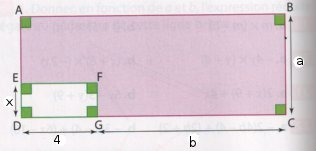
\includegraphics[width=6cm]{images/expression.jpg}
\end {center}
\end{minipage}
\end{tabular}

\bigskip


\ul{\textbf{Exercice 3:}} \textit{(3,5 points)} Pour cet exercice, on ne
demande pas de justification.

\begin{tabular}{ccc}
\begin{minipage}{6cm}
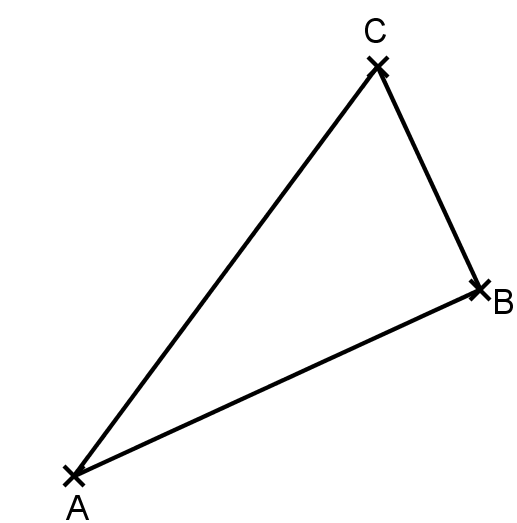
\includegraphics[width=35mm]{images/ex11.png}


\end{minipage}
&
\begin{minipage}{6cm}
\begin{center}
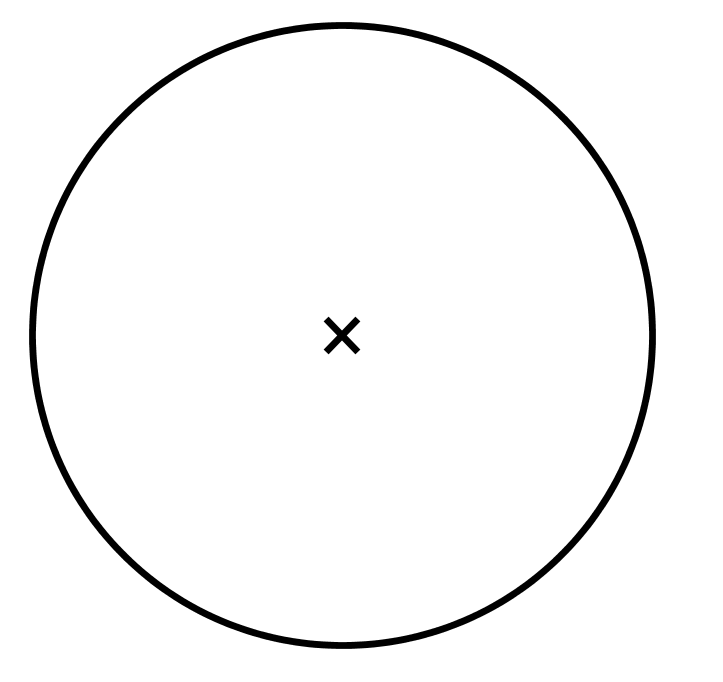
\includegraphics[width=35mm]{images/ex12.png}
\end{center}

\end{minipage}
&
\begin{minipage}{6cm}
\begin{center}
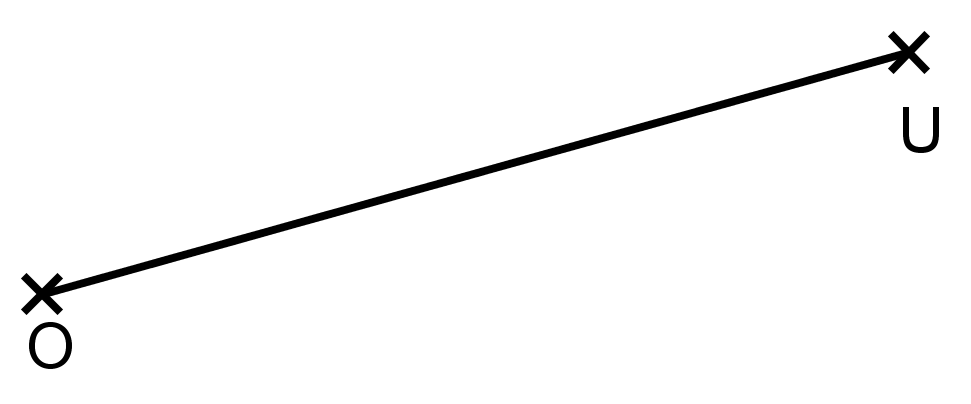
\includegraphics[width=35mm]{images/ex13.png}
\end{center}


\end{minipage} \\

\begin{minipage}{6cm}
1. Construire le cercle circonscrit 

au triangle ABC.
\end{minipage}
&
\begin{minipage}{6cm}
2. Construire un triangle DEF 

inscrit dans le cercle rectangle 

en D.
\end{minipage}
&
\begin{minipage}{6cm}
3. Construire un triangle OUI 

rectangle en I tel que UI=3cm.
\end{minipage}
\end{tabular}

 

\bigskip

\ul{\textbf{Exercice 4:}} \textit{(3 points)}

\begin{tabular}{cc}
\begin{minipage}{11cm}
\begin{enumerate}
  \item D�montrer que le triangle DEF est rectangle en D.
  \item Calculer DJ. Justifier votre r�ponse.
\end{enumerate}
\end{minipage}
&
\begin{minipage}{8cm}
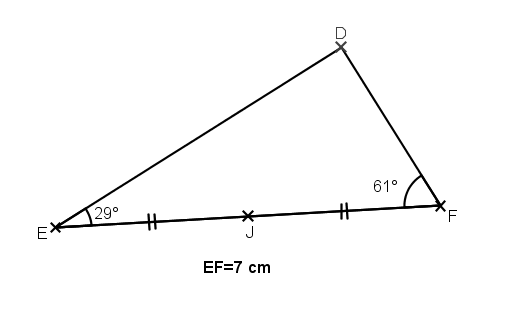
\includegraphics[width=6cm]{images/ex4.png}
\end{minipage}
\end{tabular}


\bigskip


\ul{\textbf{Exercice 5:}} \textit{(4 points)}


\begin{tabular}{cc}
\begin{minipage}{12cm}
\begin{enumerate}
  \item Quel est le centre du cercle circonscrit du triangle KOU? Justifier
  votre r�ponse.
  \item En d�duire que les points O, K, L et U appartiennent � un m�me
  cercle. Justifier votre r�ponse.
\end{enumerate}
\end{minipage}
&
\begin{minipage}{6cm}
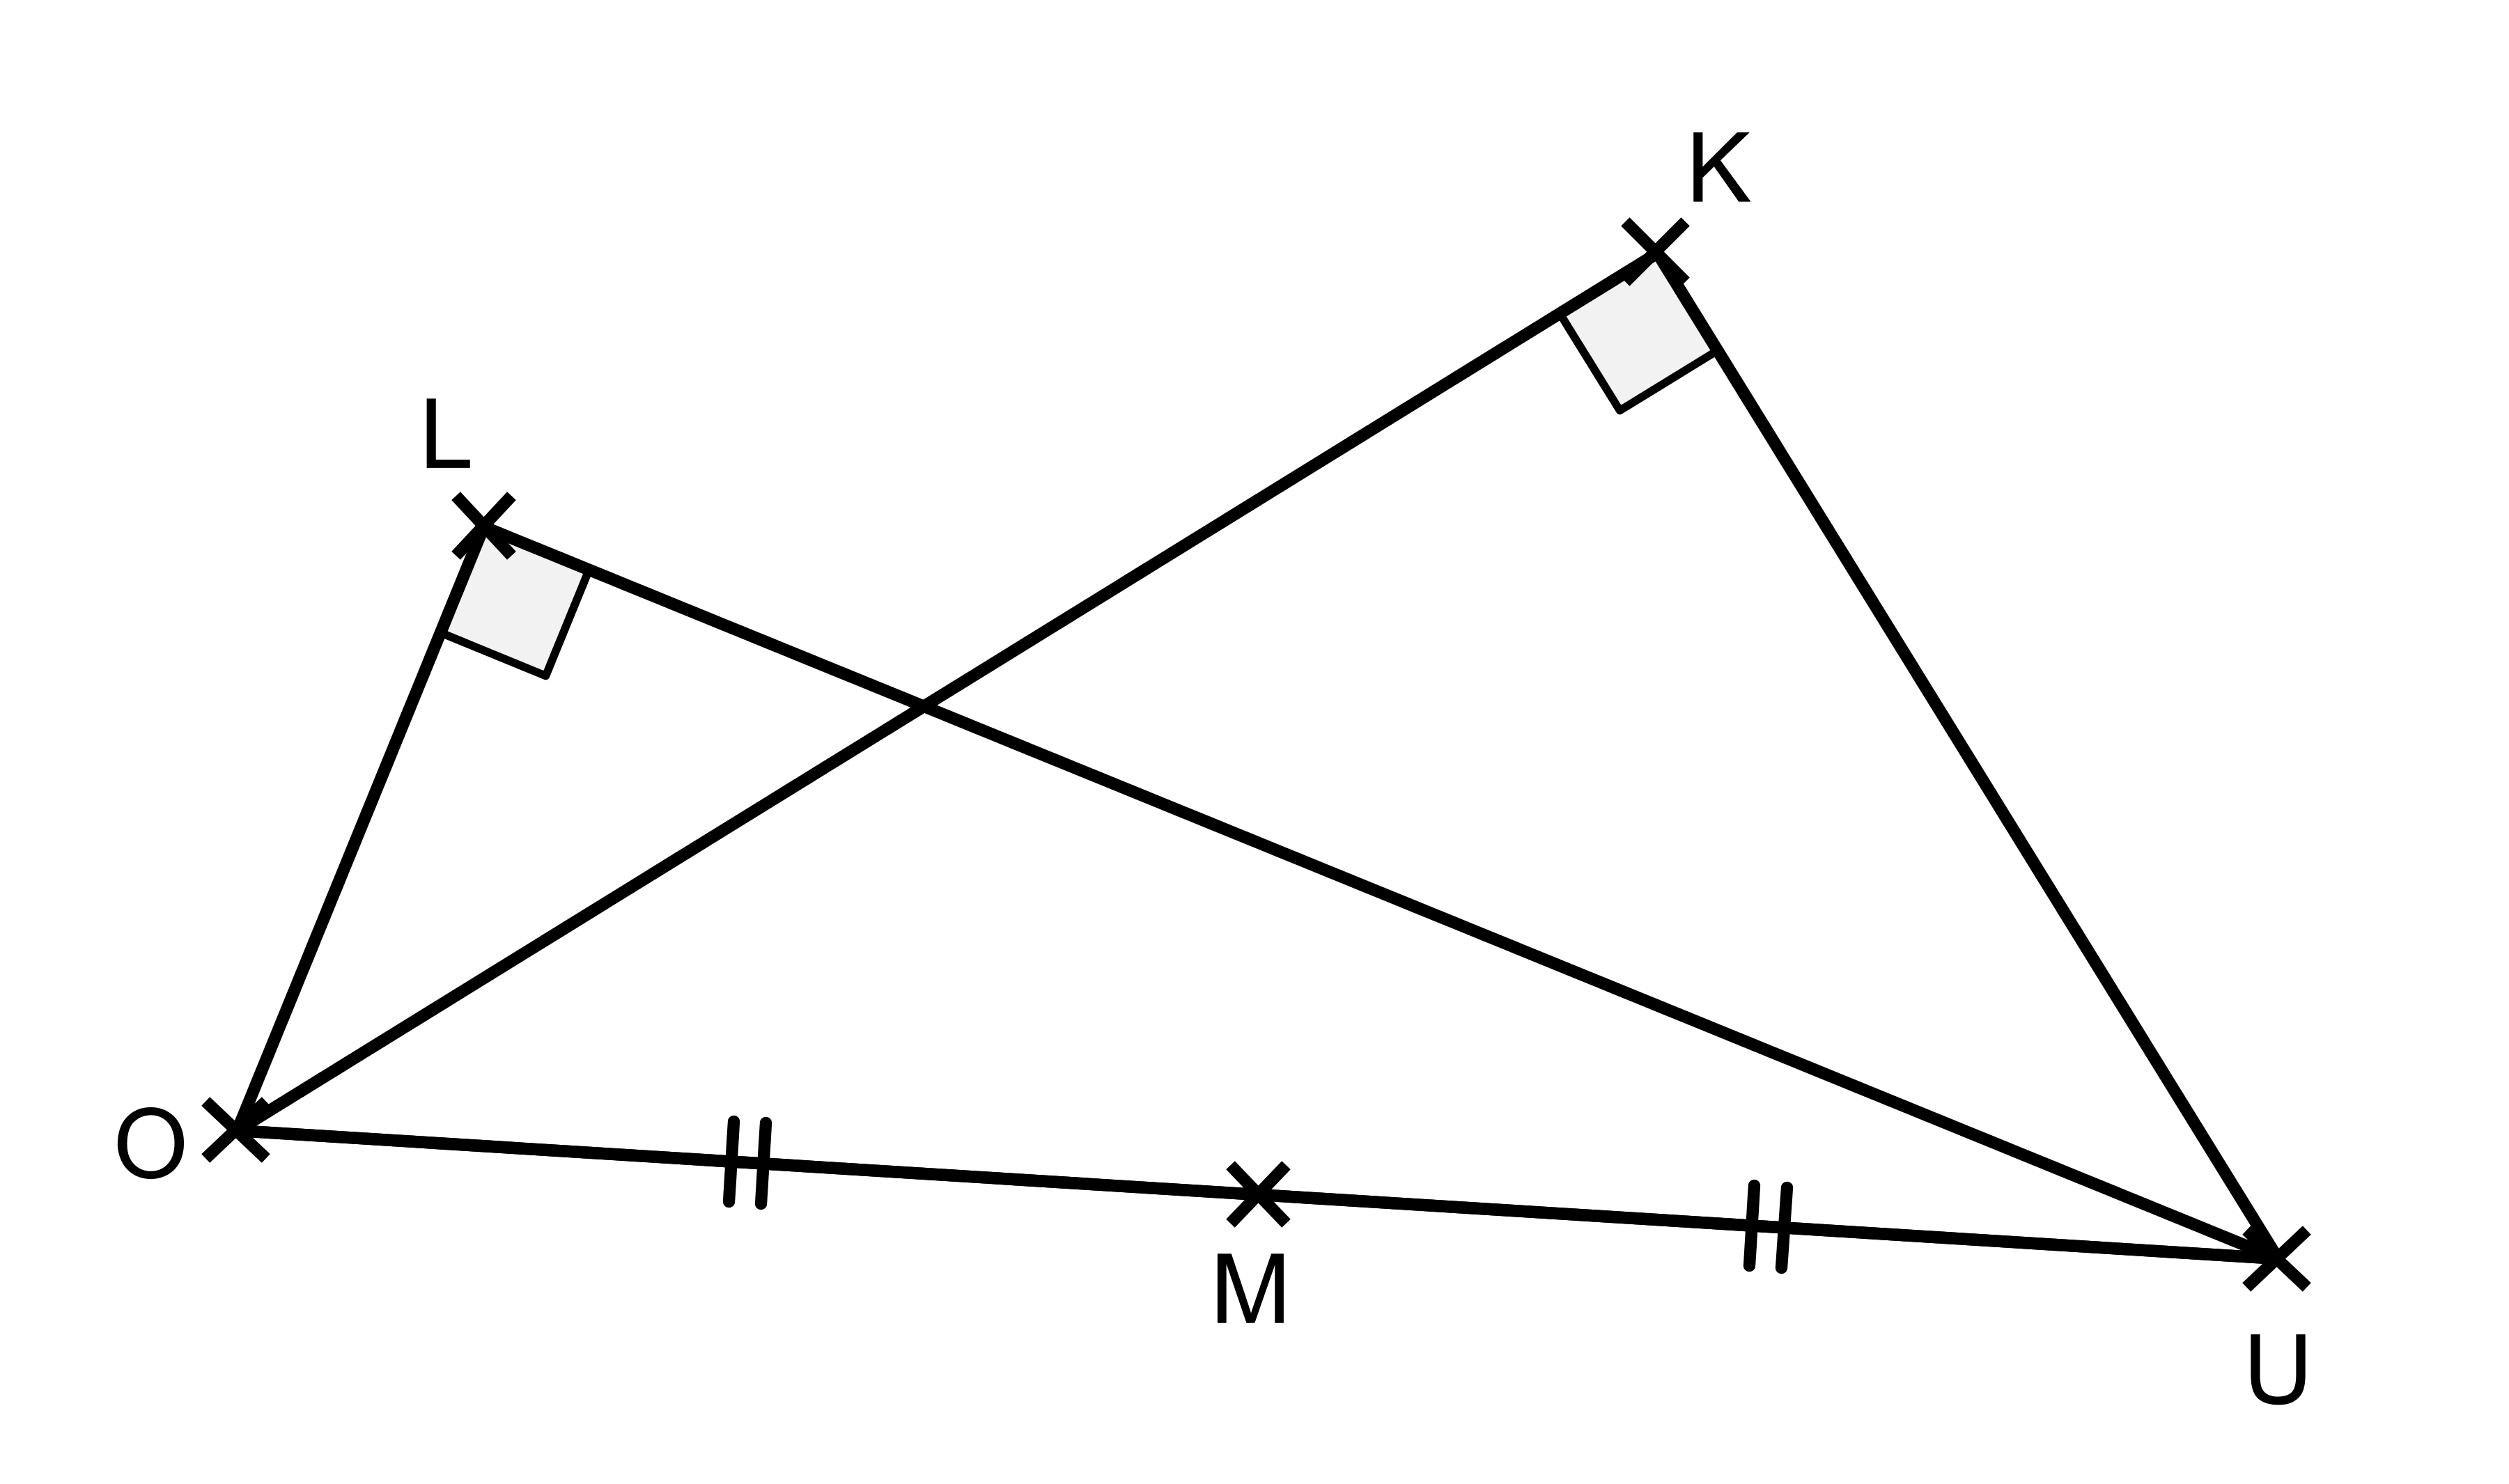
\includegraphics[width=5cm]{images/ex5.png}
\end{minipage}
\end{tabular}

\bigskip

\ul{\textbf{Exercice 6:}} \textit{(4,5 points)}


\begin{tabular}{cc}
\begin{minipage}{12cm}
\begin{enumerate}
  \item Quelle est la nature du triangle ABC? Justifier votre r�ponse.
  \item Calculer AB. Justifier votre r�ponse.
  \item Calculer $\widehat{ACB}$. Justifier votre r�ponse.
\end{enumerate}
\end{minipage} 
&
\begin{minipage}{6cm}
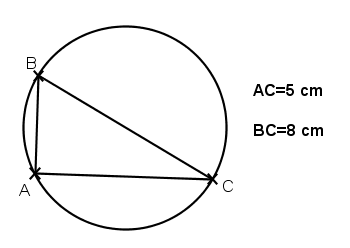
\includegraphics[width=4cm]{images/ex6.png}
\end{minipage}
\end{tabular}
\end{document}
